\newif\ifTLP\TLPtrue
\newif\ifTLPBIB%\BIBTLPtrue
\newif\ifLNCS%\LNCStrue


% TPLP/LNCS stuff

\ifTLP
  \documentclass{tlp} 
  \renewcommand{\cite}{\citep}
  \fi
\ifLNCS
  \documentclass[runningheads]{llncs}\fi

\ifTLP
  \usepackage{multirow}
\fi

% LNAI stuff

% TLP stuff

\usepackage{times}
% \usepackage{soul} % to strikeout, highline, etc.
\usepackage{url}
\usepackage[hidelinks]{hyperref}
\usepackage{graphicx}
\usepackage{booktabs}
\usepackage{algorithm}
\usepackage{algorithmic}
\urlstyle{same}
%

% OUR PACKAGES AND MACROS

\usepackage[x11names]{xcolor}

\usepackage{tikz}
\tikzset{
    event/.style={},
    smodel/.style={fill=gray!25},
    tchoice/.style={draw, circle},
    indep/.style={},
    proptc/.style = {-latex, dashed},
    propsm/.style = {-latex, thick},
    doubt/.style = {gray} }
\usetikzlibrary{calc, positioning, patterns, perspective}
%
\usepackage{hyperref}
\hypersetup{
    colorlinks=true,
    linkcolor=blue,
    citecolor=blue,
    urlcolor=blue, }
%
\usepackage{commath}
\newtheorem{assumption}{Assumption}
\usepackage{amssymb}
\usepackage[normalem]{ulem}
\usepackage[euler-digits,euler-hat-accent]{eulervm}
\usepackage[nice]{nicefrac}
\usepackage{stmaryrd}
\usepackage{acronym}
\usepackage{multicol}
\usepackage{multirow}
\usepackage{cleveref}
\crefname{example}{ex.}{exs.}
\crefname{proposition}{prop.}{props.}
\crefname{assumption}{asp.}{asps.}
\usepackage{hyphenat}
\hyphenation{
mo-dels mi-ti-ga-ted mi-ni-mal ex-am-ple spe-ci-fi-ca-tion
}

% Environments

\ifTLP
  \newtheorem{example}{Example}
  \newtheorem{definition}{Definition}
  \newtheorem{proposition}{Proposition}
\fi

% Commands

\newcommand{\eat}[1]{}
\newcommand{\at}[1]{\ensuremath{\!\del{#1}}}        %   argument
%
%   Notation
%
%   special sets
%
\newcommand{\cla}[1]{\ensuremath{{\cal #1}}}        %   class of something  
\newcommand{\clx}[1]{\ensuremath{{\mathbb{#1}}}}
%
%   connectives in logic programs
%
\newcommand{\conj}{\ensuremath{\wedge}} \newcommand{\disj}{\ensuremath{\vee}}
\newcommand{\clause}{\ensuremath{\leftarrow}}
\newcommand{\naf}{\ensuremath{\sim\!}}
\newcommand{\co}[1]{\ensuremath{\overline{#1}}}     %   complement
%
%   often used sets
%
\newcommand{\ATOMSset}{\ensuremath{\cla{A}}}
\newcommand{\LITERALSset}{\ensuremath{\cla{L}}}
\newcommand{\PATOMset}{\ensuremath{\ATOMSset_{\cla{P}}}}
\newcommand{\FACTSset}{\ensuremath{\cla{F}}}
\newcommand{\PROBFset}{\ensuremath{\cla{P}}}
\newcommand{\RULESset}{\ensuremath{\cla{R}}}
\newcommand{\TCHOICEset}{\ensuremath{\cla{T}}}
\newcommand{\MODELset}{\ensuremath{\cla{M}}}
\newcommand{\EVENTSset}{\ensuremath{\cla{E}}}
\newcommand{\CONSISTset}{\ensuremath{\cla{W}}}
%
%   often used functions
%
%   error (loss)
\newcommand{\err}[1]{\ensuremath{\mathrm{err}\at{#1}}}
%
%   probability 
\newcommand{\prfunc}{\ensuremath{\mathrm{P}}}       
%   P(X = x)
\newcommand{\pr}[1]{\ensuremath{\prfunc\at{#1}}}    
%   P_X(x)
\newcommand{\prd}[1]{\ensuremath{\prfunc_{#1}}}     
\newcommand{\prT}{\prd{\TCHOICEset}}
\newcommand{\prM}{\prd{\MODELset}}
\newcommand{\prE}{\prd{\EVENTSset}}
\newcommand{\prC}{\prd{C}}
%
%   local notation
%
 %   m(x)
\newcommand{\pw}[1]{\ensuremath{\mu\at{#1}}}           
%   m_T     total choices 
\newcommand{\pwT}{\ensuremath{\mu_{\TCHOICEset}}}   
%   m_T(x)
\newcommand{\pwt}[1]{\ensuremath{\pwT\at{#1}}}     
%   m_M     stable models  
\newcommand{\pwM}{\ensuremath{\mu_{\MODELset}}}   
%   m_M(x)
\newcommand{\pwm}[1]{\ensuremath{\pwM\at{#1}}}     
%   m_C     eq. classes 
\newcommand{\pwC}{\ensuremath{\mu_{\textrm{C}}}}   
%   m_C(x)
\newcommand{\pwc}[1]{\ensuremath{\pwC\at{#1}}}     
%   m_E     events 
\newcommand{\pwE}{\ensuremath{\mu_{\EVENTSset}}}   
%   m_E(x)
\newcommand{\pwe}[1]{\ensuremath{\pwE\at{#1}}}     
%
%
%
\newcommand{\stablecore}[1]{\ensuremath{\left\llbracket #1 \right\rrbracket}}
\newcommand{\inconsistent}{\bot}
\newcommand{\given}{\ensuremath{~\middle|~}}
\newcommand{\bottomclass}{\ensuremath{\Lambda}}
\newcommand{\indepclass}{\ensuremath{\Diamond}}
\newcommand{\probfact}[2]{\ensuremath{#1:#2}}
\newcommand{\probrule}[3]{\probfact{#1}{#2} \leftarrow #3}
\newcommand{\class}[1]{\ensuremath{[{#1}]_{\sim}}}
\newcommand{\tcgen}[1]{\MODELset\at{#1}}
\newcommand{\condsymb}[2]{\ensuremath{p_{#1|#2}}}
\newcommand{\lpmln}{\texttt{LP\textsuperscript{MLN}}}
\newcommand{\emptyevent}{\ensuremath{\lambda}}
%
%   Acronyms
%
\acrodef{BK}[BK]{background knowledge}
\acrodef{ASP}[ASP]{answer set program}
\acrodef{NP}[NP]{normal program}
\acrodef{PCR}[PCR]{program with choice rules}
\acrodef{DS}[DS]{distribution semantics}
\acrodef{PF}[PF]{probabilistic fact}
\acrodef{TC}[TC]{total choice}
\acrodef{SM}[SM]{stable model}
\acrodef{SC}[SC]{stable core}
\acrodef{KL}[KL]{Kullback-Leibler}
\acrodef{SBF}[SBF]{Simple But Fruitful}
\acrodef{RSL}[RSL]{Random Set of Literals}
\acrodef{RCE}[RCE]{Random Consistent Event}
\acrodef{SASP}[SASP]{Stochastic Answer Set Program}
%
%   Reviewing
%
\newcommand{\LOOK}{\ensuremath{\blacksquare}}
\newcommand{\delete}[1]{\sout{#1}}
\newcommand{\replace}[2]{\delete{#1}{#2}}
\newcommand{\franc}[1]{{\color{green!30!black}#1}}
\newcommand{\bruno}{\color{red!60!black}}
\newcommand{\spa}[1]{{\color{brown!80!black}{#1}}}
\newcommand{\dietmar}[1]{{\color{brown!40!black}#1}}


\begin{document}

%   PREAMBLE / METADATA

\title{%
    An Algebraic Approach to Stochastic
    Answer~Set~Programming
}
\ifTLP
  \lefttitle{F.~Coelho, B.~Dinis, D.~Seipel and S.~Abreu}

  \begin{authgrp}
    \author{\sn{Francisco} \gn{Coelho}}
    \affiliation{NOVA-LINCS, University of \'Evora}
    \email{spa@uevora.pt}

    \author{\sn{Bruno} \gn{Dinis}}
    \affiliation{CIMA, University of \'Evora}
    \email{bruno.dinis@uevora.pt}

    \author{\sn{Dietmar} \gn{Seipel}}
    \affiliation{Universit\"at W\"urzburg}
    \email{dietmar.seipel@uni-wuerzburg.de}

    \author{\sn{Salvador} \gn{Abreu}}
    \affiliation{NOVA-LINCS, University of \'Evora}
    \email{spa@uevora.pt}
  \end{authgrp}
\else
\author{%
    Francisco Coelho\inst{1,2}   \and %
    Bruno Dinis\inst{1,3}        \and %
    Dietmar Seipel\inst{4}       \and %
    Salvador Abreu\inst{1,2}     %
}
\institute{%
    University of Évora \\
    \email{\{fc,bruno.dinis,spa\}@uevora.pt} \and
    NOVA LINCS \and
    CIMA \and
    Universit\"at W\"urzburg \\
    \email{dietmar.seipel@uni-wuerzburg.de}
}

\fi
\maketitle

% \renewcommand*{\cite}[1]{(cite (#1))}
\begin{abstract}
  We address the problem of propagating the probabilities from the \spa{more, more!}
  annotated facts of an \acl{ASP} to its \aclp{SM}, and from there to
  general events in the program's domain.
  % 
  Our approach is algebraic in the sense that it relies on an
  equivalence relation over the set of events, and uncertainty is
  expressed with variables and polynomial expressions.
  % 
  We propagate probability in the space of models and events, instead
  of dealing with the syntax of the program.
  % 
  We illustrate our methods with two examples, one of which shows a
  connection to bayesian networks.
\end{abstract}

\begin{keywords}
  Answer-Set Programming, Stable Models, Probabilistic Logic Programming
\end{keywords}


\section{Introduction and Motivation}

A major limitation of logical representations in real world
applications is the implicit assumption that the \acl{BK} is perfect.
This assumption is problematic if data is affected by stochastic
factors, which is often the case.  Here we aim to explore how
\aclp{ASP} with probabilistic facts can lead to characterizations of
probability distributions on the program's domain.

Current systems such as \texttt{Problog} \cite{de2007problog},
\texttt{P-log} \cite{baral2009probabilistic} or \lpmln
\cite{lee2016weighted}, in line with \cite{kifer1992theory}, derive a
probability distribution from the \textit{syntax} of a program.
%
Instead, we propose a method where such distributions result from the
program's \textit{\acp{SM}} and probability-annotated facts.  We use
those facts to define a function on the \acp{SM} and then propagate
that function to a probability distribution of the events in the
program domain.

The step from facts to \aclp{SM} is non-deterministic in the sense
that a given set of facts entails zero, one or more \acp{SM}.  As
explained below, and also in
\cite{verreet2022inference,pajunen2021solution,cozman2020joy,baral2009probabilistic},
this poses a problem when propagating probabilities from annotated
facts to \aclp{SM}.
%
We represent some non-unique choices by a parameter that can be later
estimated from further information, \emph{e.g.}\ observations.  This
approach enables later refinement and scoring of a partial program of
a model from additional evidence.

\Acp{ASP} \cite{lifschitz2002answer,lifschitz2008twelve} are logic
programs based on the \acl{SM} semantics of \acp{NP}.  \Acp{ASP}
represent a problem and the resulting models (\emph{answer sets}) can
be found either using SAT solving technology
\cite{gebser2011potassco,adrian2018asp,niemela1997smodels} or through
top-down searching
\cite{alberti2017cplint,arias2020justifications,marple2017computing}.
Unlike \texttt{Prolog}, \ac{ASP} is a truly declarative language that
supports language constructs such as disjunction in the head of a
rule, choice rules, and both hard and weak constraints.
%
The \ac{DS} \cite{sato1995statistical,riguzzi2022foundations} is a key
approach to extend logical representations with probabilistic
reasoning.  We can foresee two key applications of this extension of
logic programs:
%
\begin{enumerate}
  % 
\item Support probabilistic reasoning tasks on the program domain,
  \textit{i.e.} the set of all events, \(\EVENTSset\).
  % 
\item Given a dataset and a divergence measure, the program can be
  scored (\textit{e.g.}\ by the divergence w.r.t.\ the \emph{empiric}
  distribution of the dataset), and weighted or sorted amongst other
  programs.  These are key ingredients in algorithms searching, for
  example, optimal models of a dataset.
  % 
\end{enumerate}

To propagate probabilities from \aclp{TC} to events we start with the
following stance:
\begin{itemize}
\item A program describes an observable system.
\item The \aclp{SM} are the possible states of that system.
\item Observations (\textit{i.e.}\ events) are stochastic.
\end{itemize}

In particular, one observation can be sub-complete (a proper subset of
a \ac{SM}) or super-complete (a proper superset of a \ac{SM}), and
might not uniquely determine the real state of the system.  From here,
probabilities must be extended from \acp{TC} to \acp{SM} and then to
any event.
%
This propagation process soon faces a non-deterministic problem,
illustrated by the example in \cref{sec:example.1}, where multiple
\acp{SM}, \(ab\) and \(ac\), result from a single \ac{TC}, \(a\), but
there is not enough explicit information in the program to assign a
single probability to each \ac{SM}.
%
We propose to use algebraic variables to describe that lack of
information and then estimate the value of those variables from
empirical data.

The lack of unique \acp{SM} is also addressed in \cite{cozman2020joy}
along a different approach, using credal sets.
%
In another related work, \cite{verreet2022inference} epistemic
uncertainty (or model uncertainty) is considered as a lack of
knowledge about the underlying model, that may be mitigated via
further observations.  This seems to presuppose a bayesian approach to
imperfect knowledge in the sense that having further observations
allows to improve/correct the model.  Indeed, that approach uses Beta
distributions on the total choices in order to be able to learn a
distribution on the events.
%
This approach seems to be specially fitted to being able to tell when
some probability lies beneath some given value.  Our approach seems to
be similar in spirit, while remaining algebraic in the way that the
propagation of probabilities is addressed.

The example in \cref{sec:example.1} uses the code available in the
project's
repository\footnote{\url{https://git.xdi.uevora.pt/fc/sasp}},
developed with the \texttt{Julia} programming language
\cite{bezanson2017julia}, and the \texttt{Symbolics}
\cite{gowda2021high} libraries.


\section{Syntax and Semantics of Stochastic ASP}
\label{sec:syntax.and.semantics}

We start this overview with the syntax and \ac{ASP} semantics of
(propositional) \aclp{NP} and then proceed to the case of
probabilistic annotations.  We setup a minimal syntax, enough to
illustrate our method to propagate probability from annotated facts to
general events, without variables, functors or relation symbols.


\paragraph{Syntax.}
% normal and choice rules answer set program

Let \(\ATOMSset\) be a finite set.
A \textit{positive literal}, or \textit{atom},
is any \(a \in \ATOMSset\)
and a \textit{negative literal} is \(\neg a\), also denoted \(\co{a}\),
for \(a\in\ATOMSset\).
A \textit{literal} is a positive or a negative literal.
A \textit{fact} is a literal.
For literals $l_1, \ldots, l_n$, a \emph{conjunction} is
  \( l _1 \conj \cdots \conj l_n, \)
and a \textit{disjunction} is
  \( l_1 \disj \cdots \disj l_n. \)
A \textit{choice rule} is of the form
   \( \alpha \clause \beta, \)
where $\alpha$ is a disjunction, the \textit{head},
and \(\beta\) a conjunction, the \textit{body}.
In a \textit{normal rule} the head is a single literal.
An \textit{\acf{ASP}} is a set of facts and
(both normal and choice) rules, denoted, resp. $\FACTSset\at{P}$ and
$\RULESset\at{P}$, or simply $\FACTSset$ and $\RULESset$.
Notice that a choice rule can be converted to a set of normal rules
\cite{gebser2022answer}.


\paragraph{Semantics.}

The standard semantics of an \ac{ASP} can have different, equivalent,
definitions \cite{lifschitz2008twelve}.  A common definition is as
follows \cite{gelfond1988stable}.  Let \(P\) be a \acl{NP}.
\franc{check the reference} The Gelfond/Lifschitz \emph{reduct} of
\(P\) relative to the set $X$ of atoms results from (i) deleting rules
that contain a literal \(\neg l\) in the body with \(l \in X\) and
then (ii) deleting remaining literals \(\neg l'\) from the bodies of
the remaining rules.  Now, \(M\) is a \textit{\acf{SM}} of \(P\) if it
is the minimal model of the reduct of \(P\) relative to \(M\).  We
denote \(\MODELset\at{P}\), or simply \(\MODELset\), the set of
\aclp{SM} of the program~ \(P\).


\paragraph{Evaluation without Grounding.}

A promising approach to handle the generation of stable models is the
one supported by \texttt{s(CASP)}, a system that can evaluate ASP
programs with function symbols (functors) and constraints without
grounding them either before or during execution, using a method
similar to SLD resolution
\cite{marple2017computing,arias2020justifications}.  This enables the
generation of human readable explanations of the results of programs
and addresses two major issues of grounding-based solvers, that %
   (1) either do not support function symbols or, using finite domains,
       lead to exponential groundings of a program and %
   (2) compute the complete model of the grounded program when, in some
       scenarios, it is desirable to compute only a partial stable model
       containing a query.
 

\subsection*{\acsp{SASP} and their Derived Programs}
%   probabilistic fact stochastic answer set programs (sasp)
%   derived program stable models 

\emph{\Acfp{SASP}} extend \ac{ASP} by adding facts with probabilistic
annotations: A \textit{\ac{PF}} is \(\probfact{a}{p}\) where \(a\) is
an atom and \(p\in\intcc{0,1}\).  We denote the set of \aclp{PF} of a
program by \(\PROBFset\), and \(\PATOMset\) the set of positive
literals in \(\PROBFset\).

\eat{\franc{Discuss probabilities in the head of rules and in
    disjunctions (?).}}%

\franc{%
  Our definition of \acp{SASP} is restricted in several ways because
  our goal here is to illustrate the core of a method to propagate
  probabilities from \aclp{TC} to events.  So these programs do not
  feature variables, relation symbols, functors or other elements
  common in standard \ac{ASP}.  Also probability annotations are not
  associated to (general) clause heads or disjunctions.  However,
  these two last restrictions do not reduce the expressive capacity of
  the language because, for the former, a clause such as
  \( \probrule{\alpha}{p}{\beta} \) with an annotated head can be
  rewritten as:
  \begin{equation*}
    \probrule{\alpha}{p}{\beta} \qquad \Longrightarrow \qquad
    \begin{aligned}
        \probfact{\gamma & }{p}, \\
        \alpha           & \clause \beta \wedge \gamma
    \end{aligned}
  \end{equation*}
  while annotated disjunctive facts, such as
    \( \probfact{\alpha \vee \beta}{p} \),
  can be replaced by
  \begin{equation*}
    \probfact{\alpha \vee \beta}{p} \qquad \Longrightarrow \qquad 
    \begin{aligned}
        \probfact{\gamma  & }{p}, \\
        \alpha \vee \beta & \clause \gamma.
    \end{aligned}
  \end{equation*}
}

\paragraph{Interpretation of an SASP.}

The \emph{derived program} of an \ac{SASP} is obtained by replacing
each \acl{PF} \(\probfact{a}{p}\) by a disjunction
   \( a \disj \co{a}. \)
The \textit{\aclp{SM}} of an \acs{SASP} program are the \aclp{SM}
of its derived program.
The set of \acp{SM} of a (derived or) \acs{SASP} program is
denoted~\(\MODELset\).

\begin{example}[Fruitful SASP]
  \label{ex:fruitful}\em Consider \(A\) to be the following \ac{SASP}:
  \begin{equation}\label{eq:fruitful}
    \begin{split}
      \probfact{a&}{0.3}, \\
      b \vee c          & \clause a
    \end{split}
  \end{equation}
  which has the set \({\cal P} = \{ a:0.3 \}\) of probabilistic
  facts.  This program is transformed into the disjunctive logic
  program
  \begin{equation}\label{eq:derived.fruitful}
    \begin{split}
      a \vee \co{a},\\
      b \vee c          & \clause a,
    \end{split}
  \end{equation}
  with the set
       \( {\cal M} = \{\, \co{a}, ab, ac\, \} \)
  of three stable models.
  We use short-hand expressions like \(ab\) to denote a set
  of literals such as \(\set{a, b}\).
  \franc{\LOOK~Consider also the case \(c \clause a\).}
\end{example}

The method we are proposing here does not follow the framework of \cite{kifer1992theory} by attributing probabilities directly from the syntax of the program. Our approach requires that we consider the semantics, \emph{i.e.}\ the \aclp{SM} of the program, no matter the syntax that provided them.

\begin{example}[No Syntax Propagation]\label{example:not.syntax.propagation}
    Consider the program
    \begin{equation*}
        \begin{split}
            \probfact{a&}{0.3}, \\
            b & \clause a
        \end{split}
    \end{equation*}
    We don't follow the clause \(b \clause a\) to attribute a probability to \(b\). Instead, that will result from considering how events are related with the \aclp{SM} and these with the \aclp{TC}. If one follows the steps of \cref{sec:propagating.probalilities} would get 
    \begin{equation*}
        \begin{split}
            \prE\at{a} & = \prE\at{b} = \prE\at{ab} = 0.05,\\
            \prE\at{\co{a}} & = \prE\at{\co{a} b} = \prE\at{\co{a}\co{b}} = \frac{7}{60},\\
            \prE\at{\set{}} & = 0.5.\\
        \end{split}
    \end{equation*}
\end{example}

\subsection*{Events}

An \emph{event} is a set of literals.
We denote the set of events by \(\EVENTSset\).
An event \(e \in \EVENTSset\) containing a set
   \(\set{x, \co{x}} \subseteq e\)
of complementary literals is \textit{inconsistent};
otherwise \(e\) is \textit{consistent}.
The set of consistent events is denoted by \(\CONSISTset\).

\begin{example}[Events of the fruitful \ac{SASP}]\label{ex:events}\em
  The atoms of program \cref{eq:fruitful} are
  \(\ATOMSset = \set{a, b, c}\) and the literals are
\begin{equation*}
   \LITERALSset = \set{\, \co{a}, \co{b}, \co{c}, a, b, c\, }.
\end{equation*}
In this case, \(\EVENTSset\) has \(2^6 = 64\) elements.  Some, such as
\(\set{\co{a}, a, b}\), contain an atom and its negation (\(a\) and
\(\co{a}\) in that case) and are inconsistent.  The set of atoms
\(\ATOMSset = \set{a, b, c}\) above generates \(37\) inconsistent
events and \(27\) consistent events.  Notice that the empty set is an
event, that we denote by \emptyevent.
    
As above, to simplify notation we write events as \(\co{a}ab\) instead
of \(\set{\co{a}, a, b}\).
\end{example}


\subsection*{Total Choices and their Probability}

A disjunctive head \(a \disj \co{a}\) in the derived program
represents a single \textit{choice}, either \(a\) or \(\co{a}\).  A
\textit{\acl{TC}} of the derived program, and of the \ac{SASP}
program, is \(t = \set{a' \given \probfact{a}{p} \in \PROBFset}\)
where each \(a'\) is either \(a\) or \(\co{a}\).  We denote by
\(\TCHOICEset\) the set of total choices of a \ac{SASP} or of its
derived program.

\begin{example}[\Aclp{PF} and \aclp{TC}]
  \label{ex:total.choices}\em \eat{\franc{Example of total choices
      with more probabilistic facts.}}
    Consider the program $B$ defined by
    \begin{equation*}
        \begin{split}
            \probfact{a&}{0.3},\\
            \probfact{b&}{0.6},\\
            c & \clause a \wedge b.
        \end{split}\label{eq:total.choices}
    \end{equation*}
    The probabilistic facts of \(B\) are
       \[ \PROBFset_{B} = \set{~\probfact{a}{0.3}, \probfact{b}{0.6}~}, \]
    and the total choices are
       \[ \TCHOICEset_{B} = \set[2]{\:
            \set[1]{a, b},
            \set[1]{a, \co{b}},
            \set[1]{\co{a}, b},
            \set[1]{\co{a}, \co{b}}\: }. \]
    E.g., the total choice \(\set{\co{a}, b} \)
    results from choosing \(a' = \co{a}\) from the probabilistic fact
    $\probfact{a}{0.3}$ and $b' = b$ from \(\probfact{b}{0.6}, \)
    while \(\set{a, b} \) results from choosing \(a' = a\) from
    \(\probfact{a}{0.3}\) and \(b' = b\) from \(\probfact{b}{0.6}\).
\end{example}

The \emph{probability of the \acl{TC} \(t \in \TCHOICEset\)} is given
by the product
\begin{equation}
    \prT\at{t} =
    \prod_{\substack{
            \probfact{a}{p}~ \in ~\PROBFset,\\
            a~ \in~ t}} p\ \ \times\
    \prod_{\substack{
            \probfact{a}{p}~ \in ~\PROBFset,\\
            \co{a}~\in~ t}} \co{p}.
    \label{eq:prob.total.choice}
\end{equation}
Here, $\co{p} = 1 - p$, and we are using the subscript in \(\prT\) to
explicitly state that this probability distribution concerns total
choices.  Later, we'll use subscripts \(\MODELset, \EVENTSset\) to
deal with distributions of \aclp{SM} and events, \(\prM, \prE\).

\begin{example}[Probabilities for \aclp{TC}]%
  \label{ex:probability.total.choices}%
  \em Continuing with the program from \cref{ex:total.choices}, the
  probabilities of the \aclp{TC} are:
  \begin{equation*}
    \begin{aligned}
            \prT\at{\set[1]{a, b}}           & = 0.3 \times 0.6           &                  & = 0.18, \\
            \prT\at{\set[1]{a, \co{b}}}      & = 0.3 \times \co{0.6}      & = 0.3 \times 0.4 & = 0.12, \\
            \prT\at{\set[1]{\co{a}, b}}      & = \co{0.3} \times 0.6      & = 0.7 \times 0.6 & = 0.42, \\
            \prT\at{\set[1]{\co{a}, \co{b}}} & = \co{0.3} \times \co{0.6} & = 0.7 \times 0.4 & = 0.28.
    \end{aligned}
  \end{equation*}
  \eat{ The total choices corresponding to the stable models of the
    program above are \( \co{a}\co{b}\co{c}, ab\co{c}, a\co{b}c. \)
    The probability of $t = \co{a}\co{b}\co{c}$ is \(0.7\) ? } %
  Suppose that in this program we change the probability in
  \(\probfact{b}{0.6}\) to \(\probfact{b}{1.0}\).  Then the \aclp{TC}
  are the same but the probabilities become
  \begin{equation*}
    \begin{aligned}
            \prT\at{\set[1]{a, b}}           & = 0.3 \times 1.0           &                  & = 0.3, \\
            \prT\at{\set[1]{a, \co{b}}}      & = 0.3 \times \co{1.0}      & = 0.3 \times 0.0 & = 0.0, \\
            \prT\at{\set[1]{\co{a}, b}}      & = \co{0.3} \times 1.0      & = 0.7 \times 1.0 & = 0.7, \\
            \prT\at{\set[1]{\co{a}, \co{b}}} & = \co{0.3} \times \co{1.0} & = 0.7 \times 0.0 & = 0.0.
    \end{aligned}
  \end{equation*}
  which, as expected from stating that \(\probfact{b}{1.0}\), is like
  having \(b\) as a (deterministic) fact:
  \begin{equation*}
    \begin{split}
            \probfact{a&}{0.3}, \\
            b &, \\
            c & \clause a \wedge b.
    \end{split}
  \end{equation*}
  This will also be stated in \cref{prop:prob.one}, when the proper
  definitions are set.
\end{example}

Some \aclp{SM} are entailed from some \aclp{TC} while other \acp{SM}
are entailed by other \acp{TC}.  We write \(\tcgen{t}\) to represent
the set of \aclp{SM} entailed by the \acl{TC} \(t \in \TCHOICEset\).

\begin{example}[\Aclp{SM} and \aclp{TC}]%
  \em Continuing \cref{ex:fruitful}, the \acl{TC} \(t = \set{\co{a}}\)
  entails a single \acl{SM}, \(\co{a}\), so
  \( \MODELset\at{\set{\co{a}}} = \set{\co{a}} \) and, for
  \(t = \set{a}\), the program has two \aclp{SM}:
  \( \MODELset\at{\set{a}} = \set{ab, ac}\).

  \begin{equation*}
    \begin{array}{l|r}
      t \in \TCHOICEset   & \MODELset\at{t} \\
      \hline \set{\co{a}} & \co{a}          \\
      \set{a}             & ab, ac
    \end{array}
  \end{equation*}
  The second case illustrates that propagating probabilities from
  \aclp{TC} to \aclp{SM} entails a non-deterministic step: \textit{How
    to propagate the probability \(\prT\at{\set{a}}\) to each one of
    the \aclp{SM} \(ab\) and \(ac\)?}
\end{example}

%
\franc{\LOOK~Repeated?~}Our goal is to propagate the probability
distribution of the program's \aclp{TC}, \(\prT\), in
\cref{eq:prob.total.choice} (which is, indeed, a product of Bernoulli
distributions \cite{Teugels90}), to a distribution of the program's
events, \(\prE\).


\subsection*{Other Approaches and Systems}

\eat{\bruno This subsection seems out of place here! \franc{~Fixed?}}

\franc{\LOOK~Repeated?~}The core problem of setting a semantic for
probabilistic logic programs is the propagation of probabilities from
\aclp{TC} to \aclp{SM} in the case of \ac{ASP} or to other types in
other logic programming modes (\emph{e.g.}\ to possible worlds in
\texttt{Problog}).

For example, the \emph{credal set} approach, in \cite{cozman2020joy},
defines \(\prT\) like in \cref{eq:prob.total.choice} but then, for
\(a \in \ATOMSset\), \(\pr{a \given t}\) is unknown but bounded by
\(\underbar{\prfunc}\at{a \given t}\) and
\(\overline{\prfunc}\at{a \given t}\), that can be explicitly
estimated from the program.

Also \texttt{Problog} \cite{fierens2015inference,verreet2022inference}
extends \texttt{Prolog} with probabilistic facts so that a program
specifies a probability distribution over possible worlds.  A
\textit{world} is a model of \(T \cup R\) where \(T\) is a total
choice and \(R\) the set of rules of a program.  The semantics is
defined only for \textit{sound} programs \cite{riguzzi2013well}
\textit{i.e.}, programs for which each possible total choice \(T\)
leads to a well-founded model that is two-valued or \textit{total}.
The probability of a possible world that is a model of the program is
the probability of the total choice.  Otherwise the probability is
\(0\) \cite{riguzzi2013well,van1991well}.

Another system, based on Markov Logic \cite{richardson2006markov}, is
\lpmln\ \cite{lee2016weighted,lee2017lpmln}, whose models result from
\textit{weighted rules} of the form \(a \clause b, n\) where \(a\)
is disjunction of atoms, \(b\) is conjunction of atoms and \(n\) is
constructed from atoms using conjunction, disjunction and negation.
For each model there is a unique maximal set of rules that are
satisfied by it and the respective weights determine the probability
of that model.


\subsection*{Towards Propagating Probabilities from Literals to Events}
\label{sec:example.1}

Probabilistic logic programs can be traced to \cite{kifer1992theory}
where the syntax of the program determines the propagation from
probabilities explicitly set either in facts or other elements of the
program.  We take a different approach, based on the semantics of a
derived program.

Consider the program in \cref{eq:fruitful} from \cref{ex:fruitful} in
order to showcase the problem of propagating probabilities from
\aclp{TC} to \aclp{SM} and then to events.  As mentioned before, the
main issue arises from the lack of information in the program on how
to assign a single probability to each \acl{SM}.  This becomes a
crucial problem in situations where multiple \aclp{SM} result from a
single \acl{TC}.

We will follow through with this example in
\cref{sec:propagating.probalilities}, where we present our proposal
for propagating probabilities from \aclp{TC} to \aclp{SM}.

\begin{example}[Probabilities and \aclp{SM}]%
  \label{running.example}%
  \em As a first step to propagate probability from \aclp{TC} to
  events, consider the program \cref{eq:fruitful} and a possible
  propagation of \(\prT:\TCHOICEset \to \intcc{0,1}\) from \aclp{TC}
  to the \aclp{SM}, \(\prM:\MODELset \to \intcc{0,1}\).

  The \aclp{SM} are the ones from its derived program (in
  \cref{eq:derived.fruitful}):
       \[ \MODELset = \set{\co{a}, ab, ac}. \]
  It might seem straightforward to assume \(\prM\at{\co{a}}=0.7\) but
  \emph{there is no explicit way to assign values to \(\prM\at{ab}\) and
    \(\prM\at{ac}\)}.  Instead, we assume this lack of information and use a
  parameter \(\theta\) as in
  \begin{equation*}
    \begin{aligned}
            \prM\at{ab} & = 0.3\, \theta, \cr
            \prM\at{ac} & = 0.3\, (1 - \theta)
    \end{aligned}
  \end{equation*}
  to express our knowledge that $ab$ and $ac$ are models related in a
  certain way and, simultaneously, our uncertainty about that
  relation.  In general, there might be necessary several such
  parameters, each associated to a \acl{SM} \(s\) and a \acl{TC}
  \(t\), so we write \(\theta=\theta_{s,t}\).

  A value for \(\theta_{s,t}\) can't be determined just with the
  information given in that program, but might be estimated with the
  help of further information, such as empirical distributions from
  datasets.
\end{example}

Our stance is that an \ac{ASP} program describes some system and then:

\begin{enumerate}
\item With a probability set for the \aclp{SM}, we extend it to any
  event in\ the program domain, \textit{i.e.}\ to any set of literals
  present in the program.

\item In the case where some statistical knowledge is available, for
  example, in the form of a distribution relating some literals, we
  consider it as ``external'' knowledge about the parameters, that
  doesn't affect the extension procedure described below.

\item That knowledge can be used to estimate parameters and to
  ``score'' the program.

\item\label{item:program.selection} If a program is but one of many
  possible candidates then that score can be used, \emph{e.g.}\ as
  fitness, by algorithms searching (optimal) programs of a dataset of
  observations.

\item If observations are not consistent with the program, then we
  ought to conclude that the program is wrong and must be changed
  accordingly.
\end{enumerate}

Currently, we are addressing the problem of propagating a probability
function (possibly using parameters such as \(\theta\) above), defined
on the \aclp{SM} of a program,
\franc{\(\prM: \MODELset \to \intcc{0,1}\)}, to all the events of that
program: \franc{\(\prE: \EVENTSset \to \intcc{0,1}\)}.  This extension
must satisfy the Kolmogorov axioms of probability so that
probabilistic reasoning is consistent with the \ac{ASP} program and
follows our interpretation of \aclp{SM} as the states of an observable
system.

As sets, the \aclp{SM} can have non-empty intersection.  But as states
of a system, we assume that the \aclp{SM} are \emph{distinct
  observations} in the following sense:

\begin{assumption}\label{assumption:smodels.disjoint}%
  \Aclp{SM} are disjoint probabilistic events. \textit{I.e.,} for any
  set \(X\) of \aclp{SM},
  \begin{equation}
        \prM\at{X} = \sum_{s\in X}\prM\at{s}
  \end{equation}
\end{assumption}

Consider the \aclp{SM} \(ab, ac\) from \cref{running.example}, that
result from the rule \(b \vee c \clause a\) and the \acl{TC}
\(\set{a}\).  Since we intend to associate each \acl{SM} with a state
of the system, \(ab\) and \(ac\) should be \emph{disjoint} events.
From that particular rule, no further relation between \(b\) and \(c\)
is entailed.  This does not prevent that other rules set further
dependencies between \(b\) and \(c\), which in turn may change the
\aclp{SM}.

By not making prior distribution assumptions based on the syntax of
the program, we can state properties on its models, as we've done in
assumption \ref{assumption:smodels.disjoint}.


\section{Propagating Probabilities}
\label{sec:propagating.probalilities}

\begin{figure}[t]
  \begin{center}
    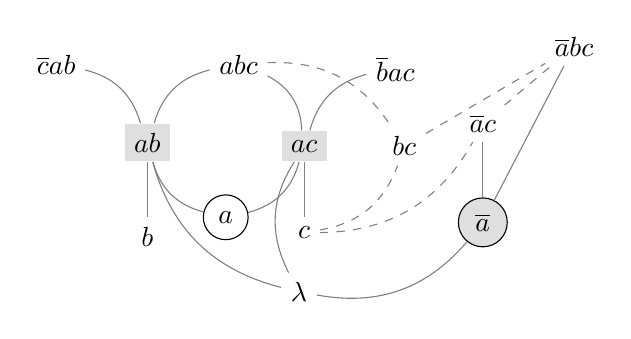
\begin{tikzpicture}[node distance=2em]
      \node[event] (E) {\(\emptyevent\)};
      \node[tchoice, above left = of E] (a) {\(a\)};
      \node[smodel, above left = of a] (ab) {\(ab\)};
      \node[smodel, above right = of a] (ac) {\(ac\)};
      \node[event, below = of ab] (b) {\(b\)};
      \node[event, below = of ac] (c) {\(c\)};
      \node[event, above right = of ab] (abc) {\(abc\)};
      \node[event, above left = of ab] (abC) {\(\co{c}ab\)};
      \node[event, above right = of ac] (aBc) {\(\co{b}ac\)};
      \node[indep, right = of ac] (bc) {\(bc\)};
      \node[tchoice, smodel, below right = of bc] (A) {\(\co{a}\)};
      \node[event, above = of A] (Ac) {\(\co{a}c\)};
      \node[event, above right = of Ac] (Abc) {\(\co{a}bc\)};
      % ----
      \draw[doubt] (a) to[bend left] (ab);
      \draw[doubt] (a) to[bend right] (ac);

      \draw[doubt] (ab) to[bend left] (abc);
      \draw[doubt] (ab) to[bend right] (abC);

      \draw[doubt] (ac) to[bend right] (abc);
      \draw[doubt] (ac) to[bend left] (aBc);

      \draw[doubt, dashed] (Ac) to (Abc);

      \draw[doubt] (A) to (Ac);
      \draw[doubt] (A) to (Abc);

      \draw[doubt] (ab) to[bend right] (E);
      \draw[doubt] (ac) to[bend right] (E);
      \draw[doubt] (A) to[bend left] (E);

      \draw[doubt] (ab) to (b);
      \draw[doubt] (ac) to (c);
      % \draw[doubt] (ab) to[bend left] (a);
      % \draw[doubt] (ac) to[bend right] (a);
      \draw[doubt, dashed] (c) to[bend right] (bc);
      \draw[doubt, dashed] (abc) to[bend left] (bc);
      \draw[doubt, dashed] (bc) to (Abc);
      \draw[doubt, dashed] (c) to[bend right] (Ac);
    \end{tikzpicture}
  \end{center}

  \caption{%
    This (partial sub-/super-set) diagram shows some events related to
    the \aclp{SM} of the program \cref{eq:fruitful}.  The circle nodes
    are \aclp{TC} and shaded nodes are \aclp{SM}.  Solid lines
    represent relations with the \aclp{SM} and dashed lines some
    sub-/super-set relations with other events.  The set of events
    contained in all \aclp{SM}, denoted by \(\bottomclass\), is
    \(\set{ \emptyevent }\) in this example, because
    \(\co{a} \cap ab \cap ac = \emptyset = \emptyevent\).}
  \label{fig:running.example}
\end{figure}

The diagram in \cref{fig:running.example} illustrates the problem of
propagating probabilities from \aclp{TC} to \aclp{SM} and then to
general events in an \emph{edge-wise} process, \emph{i.e.} where the
value in a node is defined from the values in its neighbors.  This
quickly leads to coherence problems concerning probability, with no
clear systematic approach.  For example, notice that \(bc\) is not
directly related with any \acl{SM}.  Propagating values through edges
would assign a value (\(\not= 0\)) to \(bc\) hard to justify in terms
of the semantics of the program.  Instead, we propose to base the
extension in the relation an event has with the \aclp{SM}.
%
%
%
\subsection{An Equivalence Relation}
\label{subsec:equivalence.relation}
%
%
%
\begin{figure}[t]
  \begin{center}
    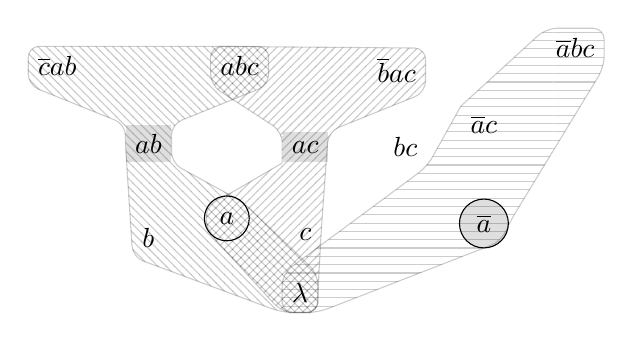
\begin{tikzpicture}[node distance=2em]
      \node[event] (E) {\(\emptyevent\)};
      \node[tchoice, above left = of E] (a) {\(a\)};
      \node[smodel, above left = of a] (ab) {\(ab\)};
      \node[smodel, above right = of a] (ac) {\(ac\)};
      \node[event, below = of ab] (b) {\(b\)};
      \node[event, below = of ac] (c) {\(c\)};
      \node[event, above right = of ab] (abc) {\(abc\)};
      \node[event, above left = of ab] (abC) {\(\co{c}ab\)};
      \node[event, above right = of ac] (aBc) {\(\co{b}ac\)};
      \node[indep, right = of ac] (bc) {\(bc\)};
      \node[tchoice, smodel, below right = of bc] (A) {\(\co{a}\)};
      \node[event, above = of A] (Ac) {\(\co{a}c\)};
      \node[event, above right = of Ac] (Abc) {\(\co{a}bc\)};
      % ----
      \path[draw, rounded corners, pattern=north west lines, opacity=0.2]
          (ab.west) -- (ab.north west) --
          % 
          (abC.south west) -- (abC.north west) -- (abC.north) --
          % 
          (abc.north east) -- (abc.east) -- (abc.south east) --
          % 
          (ab.north east) -- (ab.east) -- (ab.south east) --
          % 
          (a.north east) --
          % 
          (E.north east) -- (E.east) --
          (E.south east) -- (E.south) --
          (E.south west) --
          % 
          (b.south west) --
          % 
          (ab.west) ;
      % ----
      \path[draw, rounded corners, pattern=north east lines, opacity=0.2]
          (ac.south west) -- (ac.west) -- (ac.north west) --
          % 
          (abc.south west) -- (abc.west) -- (abc.north west) --
          % 
          (aBc.north east) -- (aBc.east) -- (aBc.south east) --
          % 
          (ac.north east) --
          % 
          (c.east) --
          % 
          (E.east) -- (E.south east) -- (E.south) -- (E.south west) --
          % 
          (a.south west) -- (a.west) -- (a.north west) -- (a.north) --
          % 
          (ac.south west) ;
      % ----
      \path[draw, rounded corners, pattern=horizontal lines, opacity=0.2]
          % (A.north west) --
          % 
          (Ac.north west) --
          % 
          (Abc.north west) -- (Abc.north) --
          (Abc.north east) -- (Abc.south east) --
          % 
          % (Ac.north east) -- (Ac.east) --
          % 
          (A.east) -- (A.south east) --
          % 
          (E.south east) -- (E.south) --
          (E.south west) -- (E.west) --
          (E.north west) --
          % 
          (bc.south east) --
          % 
          (Ac.north west) ;
    \end{tikzpicture}
  \end{center}

  \caption{Classes of (consistent) events related to the \aclp{SM} of
    \cref{ex:fruitful} are defined through sub-/super-set relations.
    In this picture we can see, for example, that
    \(\set{\co{c}ab, ab, b}\) and \(\set{a, abc}\) are part of
    different classes, represented by different fillings.  As before,
    the circle nodes are \aclp{TC} and shaded nodes are \aclp{SM}.
    Notice that \(bc\) is not in a shaded area.}
  \label{fig:running.example.classes}
\end{figure}
%
%%%%%%%%%%%%%%%%%%%%%%%%%%%%%%%%%%%%%%%%%%%%%%%%%%%%%%%%%%%%%%%%%%%%%%
%
\begin{figure}[t]
  \begin{center}
    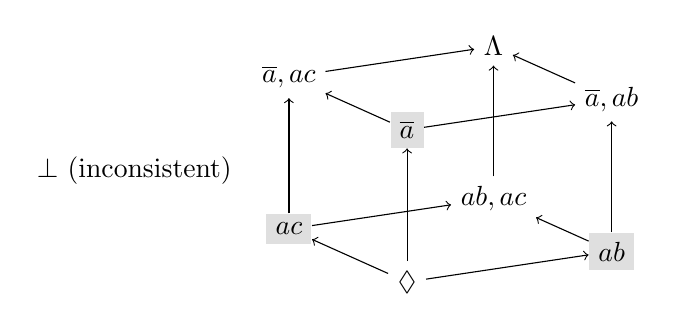
\begin{tikzpicture}[3d view]
      \node[event] (INDEPENDENT) at (0,0,0){\(\indepclass\)};
      \node[smodel] (A) at (0,0,2) {\(\co{a}\)};
      \node[smodel] (ab) at (3,0,0) {\(ab\)};
      \node[smodel] (ac) at (0,3,0) {\(ac\)};
      \node[event] (Aab) at (3,0,2) {\(\co{a},ab\)};
      \node[event] (Aac) at (0,3,2) {\(\co{a},ac\)};
      \node[event] (abac) at (3,3,0) {\(ab,ac\)};
      \node[event] (Aabac) at (3,3,2) {\(\bottomclass\)};
      \node[event] (INCONSISTENT) at (-4, 0, 2) {\(\inconsistent\)
                (inconsistent)};
      % ----
      \draw[->] (INDEPENDENT) -- (A);
      \draw[->] (INDEPENDENT) -- (ab);
      \draw[->] (INDEPENDENT) -- (ac);
      \draw[->] (A) -- (Aab);
      \draw[->] (A) -- (Aac);
      \draw[->] (ab) -- (Aab);
      \draw[->] (ab) -- (abac);
      \draw[->] (ac) -- (Aac);
      \draw[->] (ac) -- (abac);
      \draw[->] (Aab) -- (Aabac);
      \draw[->] (Aac) -- (Aabac);
      \draw[->] (abac) -- (Aabac);
    \end{tikzpicture}
  \end{center}

  \caption{%
    Lattice of the \aclp{SC} from \cref{ex:fruitful}.  In this diagram
    the nodes are the different \aclp{SC} that result from the
    \aclp{SM} plus the \emph{inconsistent} class (\(\inconsistent\)).
    The bottom node (\(\indepclass\)) is the class of
    \emph{independent} events, those that have no sub-/super-set
    relation with the \acp{SM} and the top node (\(\bottomclass\))
    represents events related with all the \acp{SM}.  As in previous
    diagrams, shaded nodes represent the \acp{SM}.}
  \label{fig:fruitful.lattice}
\end{figure}

Our path to propagate probabilities starts with a perspective of
\aclp{SM} as playing a role similar to \emph{prime factors}
\franc{\LOOK~or \emph{principal ideals}}.  The \aclp{SM} of a program
are the irreducible events entailed from that program and any event
must be considered under its relation with the \aclp{SM}.

From \cref{running.example} and \cref{fig:running.example.classes}
consider the \aclp{SM} \(\co{a}, ab, ac\) and events \(a, abc\) and
\(c\).  While \(a\) is related with (contained in) both \(ab, ac\),
the event \(c\) is related only with \(ac\).  So, \(a\) and \(c\) are
related with different \aclp{SM}.  On the other hand, \(abc\) contains
both \(ab, ac\).  So \(a\) and \(abc\) are related with the same
\aclp{SM}.

The \textit{\acf{SC}} of the event \(e\in \EVENTSset\) is
\begin{equation}
    \stablecore{e} := \set{\, s \in \MODELset \given s \subseteq e \vee e \subseteq s\, } \label{eq:stable.core}
\end{equation}
where \(\MODELset\) is the set of \aclp{SM}.

Observe that the minimality of \aclp{SM} implies that either \(e\) is
a \acl{SM} or at least one of
$\exists s \del{s \subseteq e}, \exists s \del{e \subseteq s}$ is
false \emph{i.e.,}\ no \acl{SM} contains another.

\begin{example}[Stable cores]
\label{ex:stable.cores}\em
Continuing \cref{ex:fruitful}, depicted in
\cref{fig:running.example,fig:running.example.classes,fig:fruitful.lattice},
and \(\MODELset = \set{ab, ac, \co{a}}\), consider the following
\aclp{SC} of some events:
\begin{equation*}
  \begin{aligned}
            \stablecore{a}         & = \set{s \in \MODELset \given s \subseteq a \vee a \subseteq s}                                        & = \set{ab, ac} \\
            \stablecore{abc}       & = \set{s \in \MODELset \given s \subseteq abc \vee abc \subseteq s}                                    & = \set{ab, ac} \\
            \stablecore{\co{c}ab}  & = \set{s \in \MODELset \given s \subseteq \co{c}ab \vee \co{c}ab \subseteq s}                          & = \set{ab}     \\
            \stablecore{bc}        & = \set{s \in \MODELset \given s \subseteq bc \vee bc \subseteq s}                                      & = \emptyset    \\
            \stablecore{\emptyevent} & = \set{s \in \MODELset \given s \subseteq \emptyset \vee \emptyset \subseteq s} = \set{ab, ac, \co{a}} & = \bottomclass \\
  \end{aligned}
\end{equation*}
Events \(a\) and \(abc\) have the same \ac{SC}, while \(\co{c}ab\) has
a different \ac{SC}.  Also, \(bc\) is \emph{independent of}
(\emph{i.e.}\ not related to) any \acl{SM}.  Since events are sets of
literals, the empty set is an event and a subset of any \ac{SM}.
\end{example}

We now define an equivalence relation so that two events are related
if either both are inconsistent or both are consistent and, in the
latter case, with the same \acl{SC}.

\begin{definition}\label{def:equiv.rel}
  For a given program, let $u, v \in \EVENTSset$.  The equivalence
  relation \(\sim\) is defined by
  \begin{equation}
        u \sim v\ :\clause\ u,v \not\in\CONSISTset \vee \del{u,v \in \CONSISTset \wedge \stablecore{u} = \stablecore{v}}.\label{eq:equiv.rel}
  \end{equation}
\end{definition}
This equivalence relation defines a partition on the set of events,
where each class holds a unique relation with the \aclp{SM}.  In
particular we denote each class by
\begin{equation}
    \class{e} =
    \begin{cases}
        \inconsistent := \EVENTSset \setminus \CONSISTset
         & \text{if~} e \in \EVENTSset \setminus \CONSISTset, \\
        \set{u \in \CONSISTset \given \stablecore{u} = \stablecore{e}}
         & \text{if~} e \in \CONSISTset.
    \end{cases}\label{eq:event.class}
\end{equation}

\franc{
\begin{proposition}[Bottom class]\label{prop:bottom.class}
  If we denote by \(\emptyevent\) the empty set as an event, and by
  \(\bottomclass\) the class (the \emph{bottom class}) of events
  related with all the \aclp{SM}, then
    \begin{equation}
        \class{\emptyevent} = \stablecore{\MODELset} = \bottomclass.
    \end{equation}    
\end{proposition}
}

The combinations of the \aclp{SM}, together with the set of
inconsistent events (\(\inconsistent\)) form a set of representatives.

\begin{example}[Events classes]\label{ex:classes}\em
    %    
  Consider again \cref{ex:fruitful}.  As previously stated, the
  \aclp{SM} are the elements of \(\MODELset = \set{\co{a}, ab, ac}\)
  so the quotient set of this relation is
    \begin{equation*}
        \class{\EVENTSset} = \set{
            \begin{array}{lll}
                \inconsistent,           &
                \indepclass,             &
                \stablecore{\co{a}},       \\
                \stablecore{ab},         &
                \stablecore{ac},         &
                \stablecore{\co{a}, ab},   \\
                \stablecore{\co{a}, ac}, &
                \stablecore{ab, ac},     &
                \bottomclass
            \end{array}
        },
    \end{equation*}
    where \(\indepclass\) denotes the class of \emph{independent
      events} \(e\) such that \(\stablecore{e} = \set{\emptyset}\),
    while \(\bottomclass = \stablecore{\MODELset}\) is the set of
    events related with all \acp{SM}.  We have:
    %\note{Remark the odd nature of \(\bottomclass\).} EDIT:fc fix columns width
    %
    \begin{equation*}
        \begin{array}{l|lr}
            \stablecore{e}
             & \class{e}
             & \# \class{e}                                                                       \\
            \hline
            %
            \inconsistent
             & \co{a}a, \ldots
             & 37                                                                                 \\
            %
            \indepclass
             & \co{b}, \co{c}, bc, \co{b}a, \co{b}c, \co{bc}, \co{c}a, \co{c}b, \co{bc}a
             & 9                                                                                  \\
            %
            \co{a}
             & \co{a}, \co{a}b, \co{a}c, \co{ab}, \co{ac}, \co{a}bc, \co{ac}b, \co{ab}c, \co{abc}
             & 9                                                                                  \\
            %
            ab
             & b, ab, \co{c}ab
             & 3                                                                                  \\
            %
            ac
             & c, ac, \co{b}ac
             & 3                                                                                  \\
            %
            \co{a}, ab
             &
             & 0                                                                                  \\
            %
            \co{a}, ac
             &
             & 0
            %
            \\
            %
            ab, ac
             & a, abc
             & 2                                                                                  \\
            %
            \bottomclass
             & \emptyevent
             & 1
             \\
            %
            \hline \class{\EVENTSset}
             & \EVENTSset
             & 64
        \end{array}
    \end{equation*}

    Notice that \(bc \in \indepclass\), as hinted by
    \cref{fig:running.example,fig:running.example.classes}.
\end{example}

Since all events within an equivalence class have the same relation
with a specific set of \aclp{SM}, we are interested in functions,
including probability, that are constant within classes.
%
\franc{
A function \(f:\EVENTSset\to Y\), where \(Y\) is any set, is \emph{coherent} if
    \begin{equation}
        \forall u\in \class{e} \left( f\at{u} = f\at{e} \right).
    \end{equation}
}

\noindent\franc{\LOOK~Adopt the term ``coherent'' on the following text.}

In the specific case of \cref{eq:fruitful}, instead of dealing with
the \(64 = 2^6\) events, we need to consider only the \(9 = 2^3 + 1\)
classes, well defined in terms of combinations of the \aclp{SM}, to
define coherent functions.


\subsection{From \aclp{TC} to events}
\label{subsec:from.tchoices.to.events}

Our path to set a distribution on \(\EVENTSset\) starts with the more
general problem of extending \emph{measures}, since extending
\emph{probabilities} easily follows by means of a suitable
normalization (done in
\cref{eq:measure.events.unconditional,eq:probability.event}), and has
two phases:

\begin{enumerate}
\item Propagation of the probabilities, \emph{as measures}, from the
  \aclp{TC} to events.
\item Normalization of the measures on events, recovering a
  probability.
\end{enumerate}

The ``propagation'' phase, traced by \cref{eq:prob.total.choice} and
\crefrange{eq:measure.tchoice}{eq:measure.events}, starts with the
measure (probability) of \aclp{TC}, \(\pwt{t} = \prT\at{t}\),
propagates it, as a \emph{measure}, to the \aclp{SM}, \(\pwm{s}\), and
then, within the equivalence relation from \cref{eq:equiv.rel}, to a
coherent measure of events, \(\pwe{e}\), including (consistent)
worlds.  So we are setting a sequence of functions
\begin{equation*}
    \pwT \longrightarrow \pwM \longrightarrow \pwC \longrightarrow \pwE
\end{equation*}
on successive larger domains
\begin{equation*}
    \TCHOICEset \longrightarrow \MODELset \longrightarrow \class{\EVENTSset} \longrightarrow \EVENTSset
\end{equation*}
so that the last function (\(\pwE\)) is a finite coherent measure on
the set of events and thus, as a final step, it can easily define a
probability distribution of events by normalization:
\begin{equation*}
    \pwE \longrightarrow \prE.
\end{equation*}


\subsubsection*{\Aclp{TC}.}

Using \cref{eq:prob.total.choice}, for \(t \in \TCHOICEset\),
\begin{equation}
    \pwt{t} := \prT\at{t}=
    \prod_{\substack{
            \probfact{a}{p}~ \in ~\PROBFset,\\
            a~ \in~ t}} p\ \ \times\
    \prod_{\substack{
            \probfact{a}{p}~ \in ~\PROBFset,\\
            \co{a}~\in~ t}} \co{p}.
    \label{eq:measure.tchoice}
\end{equation}


\subsubsection*{\Aclp{SM}.}

Recall that each \acl{TC} \(t \in \TCHOICEset\), together with the
rules and the other facts of a program, defines the set \tcgen{t} of
\aclp{SM} associated with that choice.  Given a \acl{TC}
\(t \in \TCHOICEset\), a \acl{SM} \(s \in \MODELset \), and variables
or values \(\theta_{s,t} \in \intcc{0, 1}\) such that
\(\sum_{s\in \tcgen{t}} \theta_{s,t} = 1\), we define
\begin{equation}
    \pwm{s, t} := \begin{cases}
        \theta_{s,t} & \text{if~} s \in \tcgen{t}\cr 0 & \text{otherwise.}
    \end{cases}
    \label{eq:measure.stablemodel}
\end{equation}

The \(\theta_{s,t}\) parameters in \cref{eq:measure.stablemodel}
express the \emph{program's} lack of information about the measure
assignment, when a single \acl{TC} entails more than one \acl{SM}.  We
propose to address this problem by assigning a possibly unknown
parameter (\(\theta_{s,t}\)) conditional on the \acl{TC} (\(t\)) to
each \acl{SM} (\(s\)).  This allows the expression of a quantity that
does not result from the program but might be determined or estimated
given more information, \textit{e.g.} observed data.

\franc{
    \begin{example}[\Aclp{SM} and parameters]%
      \label{ex:models.parameters}%
      \em %
      The program from \cref{ex:fruitful} has no information about the
      probabilities of the \aclp{SM} that result from the \acl{TC}
      \(t = \set{a}\).  These models are
      \(\MODELset\at{\set{a}} = \set{ab, ac}\) so we need two
      parameters
      \(\theta_{ab, \set{a}}, \theta_{ac, \set{a}} \in \intcc{0,1}\)
      and such that (\textit{cf.}\ \cref{eq:measure.stablemodel})
        \begin{equation*}
            \theta_{ab, \set{a}} + \theta_{ac, \set{a}} = 1.
        \end{equation*}
        If we let \(\theta = \theta_{ab, \set{a}}\) then
        \begin{equation*}
            \theta_{ac, \set{a}} = 1 - \theta = \co{\theta}.
        \end{equation*}
        Also
        \begin{equation*}
            \begin{split}
                \theta_{ab, \set{\co{a}}} &= 0,\\
                \theta_{ac, \set{\co{a}}} &= 0
            \end{split}
        \end{equation*}
        because \(ab, ac \not\in\MODELset\at{\co{a}}\).
    \end{example}
}

\subsubsection*{Classes.}
\label{sssec:propagation.class.cases}

Each class is either the inconsistent class (\(\inconsistent\)) or is
represented by a \acl{SC}, \textit{i.e.}\ a set of \aclp{SM}.

\begin{description}
  %
  \item[Inconsistent class.] The inconsistent class contains events that are logically inconsistent, thus should never be observed and thus have measure zero:
        \begin{equation}
            \pwc{\inconsistent, t} := 0.
            \footnote{This measure being zero is independent of the \acl{TC}.}
            \label{eq:measure.class.inconsistent}
        \end{equation}
        %
  \item[Independent class.] An event related with no \acl{SM} corresponds to a non-state, according to the program.  So the respective measure is also set to zero:
        \begin{equation}
            \pwc{\indepclass, t} := 0.
            \label{eq:measure.class.independent}
        \end{equation}
        %
  \item[Other classes.] For the propagation function to be coherent, it must be constant within a class, its value dependent only on the \acl{SC}, and respect assumption \ref{assumption:smodels.disjoint} (\textit{i.e.}\ \aclp{SM} are disjoint probabilistic events):
        \begin{equation}
            \pwc{\class{e}, t} := \pwm{\stablecore{e}, t} = \sum_{s\in\stablecore{e}}\pwm{s, t}
            \label{eq:measure.class.other}
        \end{equation}
        and we further define
        \begin{equation}
            \pwc{\class{e}} := \sum_{t \in \TCHOICEset} \pwc{\class{e}, t}\pwt{t}.
            \label{eq:measure.class.unconditional}
        \end{equation}
        \Cref{eq:measure.class.other} states that the measure of a class \(\class{e}\) is the sum over its \acl{SC} (\(\stablecore{e}\)) and \cref{eq:measure.class.unconditional} \emph{marginalizes} \cref{eq:measure.class.other} over the \aclp{TC}.
        %
\end{description}

\franc{
  \begin{example}[Measure of \aclp{SM} and classes]\label{ex:measures.sm}\em
      \begin{equation*}
          \begin{array}{c||l|ccc|ccc|c|c|r}
              %=====================================================
                &
              A & B                                         & C      & D           & E & F & G & H & I & J
              \\[3pt]
              \hline
              \hline
              \multirow{3}{*}{\phantom{2em}}
                & \multirow{3}{*}{\stablecore{e}}
                & \multicolumn{3}{c|}{\pwm{s,\set{\co{a}}}}
                & \multicolumn{3}{c|}{\pwm{s,\set{a}}}
                & \pwc{\class{e},\set{\co{a}}}
                & \pwc{\class{e},\set{a}}
              %  & \multicolumn{3}{c|}{\pwm{s, \co{a}}}
              %  & \multicolumn{3}{c|}{\pwm{s, a}}
              %  & \pwc{\class{e}, \co{a}}
              %  & \pwc{\class{e}, a}
                & \multirow{3}{*}{\pwc{\class{e}}}
              \\[2pt]
              %=====================================================
                &
                & \co{a}                                    & ab     & ac
                & \co{a}                                    & ab     & ac
                & \pwt{\set{\co{a}}}
                & \pwt{\set{a}}
                &
              \\[2pt]
              %=====================================================
                &
                & 1                                         & 0      & 0
                & 0                                         & \theta & \co{\theta}
                & 0.7
                & 0.3
                &
              \\[3pt]
              %=====================================================
              \hline
              1
                & \co{a}
              % & \boxed{1}                           & 0              & 0
              % & \boxed{0}                           & \theta         & \co{\theta}
                & 1                                         &        &
                & 0                                         &        &
                & 1
                & 0
                & 0.7
              \\[2pt]
              %=====================================================
              %
              2
                & ab
                &                                           & 0      &
                &                                           & \theta &
                & 0
                & \theta
                & 0.3\theta
              \\[2pt]
              %=====================================================
              %
              3
                & ac
                &                                           &        & 0
                &                                           &        & \co{\theta}
                & 0
                & \co{\theta}
                & 0.3\co{\theta}
              \\[2pt]
              %=====================================================
              %
              4
                & \co{a}, ab
                & 1                                         & 0      &
                & 0                                         & \theta &
                & 1
                & \theta
                & 0.7 + 0.3\theta
              \\[2pt]
              %=====================================================
              %
              5
                & \co{a}, ac
                & 1                                         &        & 0
                & 0                                         &        & \co{\theta}
                & 1
                & \co{\theta}
                & 0.7 + 0.3\co{\theta}
              \\[2pt]
              %=====================================================
              %
              6
                & ab, ac
                &                                           & 0      & 0
                &                                           & \theta & \co{\theta}
                & 0
                & \theta + \co{\theta} = 1
                & 0.3
              \\[2pt]
              %=====================================================
              %
              7
                & \bottomclass
                & 1                                         & 0      & 0
                & 0                                         & \theta & \co{\theta}
                & 1
                & \theta + \co{\theta} = 1
                & 1
              %=====================================================
          \end{array}
      \end{equation*}

      Continuing \cref{ex:fruitful}, we show the propagation of \(\pwT\) to \(\pwM\) (\cref{eq:measure.tchoice}) and then to \(\pwC\) (\cref{eq:measure.class.other,eq:measure.class.unconditional}). The table above resumes the calculations to compute \(\pwc{\class{e}}\) for each \(e \in \EVENTSset\). For example, \(e = abc\) the calculation of \(J6 = \pwc{\class{abc}}\) follows these steps:
      \begin{enumerate}
          \item \(\stablecore{abc} = \set{ab,ac}\) --- is in line \(6\) of the table.
          \item Since \(\TCHOICEset = \set{\set{a}, \set{\co{a}}}\), we need to calculate \(I6 = \pwc{\class{abc}, \set{a}}\) and \(H6 = \pwc{\class{abc}, \set{\co{a}}}\). By \cref{eq:measure.class.other}:
                \begin{equation*}
                    \begin{aligned}
                        H6 = \pwc{\class{abc}, \set{\co{a}}} & = \sum_{s \in \stablecore{abc}} \pwm{s, \set{\co{a}}}
                        =                                    & \pwm{ab, \set{\co{a}}} +  \pwm{ac, \set{\co{a}}}      \\
                        I6 = \pwc{\class{abc}, \set{a}}      & = \sum_{s \in \stablecore{abc}} \pwm{s, \set{a}}
                        =                                    & \pwm{ab, \set{a}} +  \pwm{ac, \set{a}}
                    \end{aligned}
                \end{equation*}
          \item The \(\pwm{s,t}\) above result from \cref{eq:measure.stablemodel} --- the non-empty cells in columns \(B:D\) and \(E:G\):
                \begin{equation*}
                    \begin{aligned}
                        C6 & = \pwm{ab, \set{\co{a}}} & = 0           \\
                        D6 & = \pwm{ac, \set{\co{a}}} & = 0           \\
                        F6 & = \pwm{ab, \set{a}}      & = \theta      \\
                        G6 & = \pwm{ac, \set{a}}      & = \co{\theta}
                    \end{aligned}
                \end{equation*}
          \item So we have --- columns \(H, I\):
                \begin{equation*}
                    \begin{aligned}
                        H6 & = \pwc{\class{abc}, \set{\co{a}}} & = 0 + 0                &  & = 0 \\
                        I6 & = \pwc{\class{abc}, \set{a}}      & = \theta + \co{\theta} &  & = 1
                    \end{aligned}
                \end{equation*}
          \item At last, by \cref{eq:measure.class.unconditional} --- columns \(H, I\) and \(J\):
                \begin{equation*}
                    \begin{split}
                        J6 = \pwc{\class{abc}} &= \sum_{t\in\MODELset} \pwc{\class{abc}, t}\pwt{t} \\
                        &=  \pwc{\class{abc}, \set{\co{a}}}\pwt{\set{\co{a}}} +
                        \pwc{\class{abc}, \set{a}}\pwt{\set{a}}  \\
                        &=  0 \co{\theta} +  1 \theta =  0 \times 0.7 +  1\times 0.3 = 0.3
                    \end{split}
                \end{equation*}
      \end{enumerate}
  \end{example}
}
%
\subsubsection*{Events and probability.}\label{sssec:propagation.event.cases}

Each (non-inconsistent) event \(e \in \EVENTSset\) is in the class defined by its \acl{SC}, \(\stablecore{e}\).  So, denoting by $\# X$ the number of elements in \(X\), we set:
\begin{equation}
  \pwe{e, t} :=
  \begin{cases}
      \frac{\pwc{\class{e}, t}}{\# \class{e}} & \text{if~}\# \class{e} > 0, \\
      0                                       & \text{otherwise}.
  \end{cases}
  \label{eq:measure.events}
\end{equation}
and
\begin{equation}
  \pwe{e} := \sum_{t\in\TCHOICEset} \pwe{e, t} \pwt{t}.
  \label{eq:measure.events.unconditional}
\end{equation}

\eat{
    \franc{\LOOK~\textbf{repeated?}~The \(\theta_{s,t}\) parameters in \cref{eq:measure.stablemodel} express the \emph{program's} lack of information about the measure assignment, when a single \acl{TC} entails more than one \acl{SM}.  In that case, how to distribute the respective measures? Our proposal to address this problem consists in assigning a parameter, \(\theta_{s,t}\), conditional on the \acl{TC}, \(t\), to each \acl{SM} \(s\).  This approach allows the expression of an unknown quantity and future estimation, given more information, \textit{e.g.} observed data.
    }
}

The \emph{normalizing factor} is:

\begin{equation}
    Z :=
    \sum_{e \in \EVENTSset} \pwe{e} =
    \sum_{\class{e} \in \class{\EVENTSset}} \pwc{\class{e}},\label{eq:normalizing.factor}
\end{equation}

and now \cref{eq:measure.events.unconditional} provides a
straightforward way to define the \emph{probability of (observing) a
  single event $e \in \EVENTSset$}:

\begin{equation}
    \prE\at{e} := \frac{\pwe{e}}{Z}.\label{eq:probability.event}
\end{equation}

\Cref{eq:probability.event} defines a coherent \emph{prior}
probability of events and, together with external statistical
knowledge, can be used to learn about the \emph{initial} probabilities
of the literals, that should not (and by \cref{prop:two.distributions}
can't) be confused with the explicit \(\pwT\) set in the program.

\franc{
\begin{example}[Coherent probability of events]\label{ex:choerent.probability}\em
    
  In \cref{ex:measures.sm} we determined \(\pwc{\class{e}, t}\) from
  \cref{eq:measure.class.other} and also \(\pwc{\class{e}}\), the
  measure of each class, using \cref{eq:measure.class.unconditional},
  that marginalizes the \aclp{TC}.

    \begin{equation*}
        \begin{array}{l|cc|c|c}
            \stablecore{e}
                & \hspace{1em}\pwC\hspace{1em}
                & \hspace{1em}\#\class{e}\hspace{1em}
                & \hspace{1em}\pwE\hspace{1em}
                & \hspace{1em}\prE\hspace{1em}
            \\
            \hline
            %
            \inconsistent
                & 0
                & 37
                & 0
                & 0                           
            \\[4pt]
            %
            \indepclass
                & 0
                & 9
                & 0
                & 0                           
            \\[4pt]
            %
            \co{a}
                & \frac{7}{10}
                & 9
                & \frac{7}{90}
                & \frac{7}{207}
            \\[4pt]
            %
            ab
                & \frac{3}{10}\theta
                & 3
                & \frac{1}{10}\theta
                & \frac{1}{23}\theta
            \\[4pt]
            %
            ac
                & \frac{3}{10}\co{\theta}
                & 3
                & \frac{1}{10}\co{\theta}
                & \frac{1}{23}\co{\theta}
            \\[4pt]
            %
            \co{a}, ab
                & \frac{7 + 3\theta}{10}
                & 0
                & 0
                & 0
            \\[4pt]
            %
            \co{a}, ac
                & \frac{7 + 3\co{\theta}}{10}
                & 0
                & 0
                & 0
            %
            \\[4pt]
            %
            ab, ac
                & \frac{3}{10}
                & 2
                & \frac{3}{20}
                & \frac{3}{46}
            \\[4pt]
            %
            \bottomclass
                & 1
                & 1
                & 1
                & \frac{10}{23}
            \\[4pt]
            %
            \hline
            &&&&
            \\[-0.5em]
                & Z = \frac{23}{10}
                &
                & \frac{\pwC}{\#\class{e}}
                & \frac{\pwE}{X}
            %& \Sigma = 1 
        \end{array}
    \end{equation*}

    
    From there we can follow \cref{eq:measure.events} to calculate the
    measure \(\pwe{e, t}\) of each event given \(t\), by simply
    dividing \(\pwc{\class{e}, t}\) by \(\#\class{e}\), the total
    number of elements in \(\class{e}\).  Then we marginalize \(t\) in
    \(\pwe{e, t}\) to get \(\pwe{e}\).  Finally, the normalization
    factor from \cref{eq:normalizing.factor} and
    \cref{eq:probability.event} provide a coherent \emph{prior}
    probability for each event.

    In summary, the coherent \emph{prior} probability of events of
    program \cref{eq:fruitful} is
    \begin{equation}
        \begin{array}{l|ccccccccc}
            \stablecore{e}          &
            \inconsistent           &
            \indepclass             &
            \co{a}                  &
            ab                      &
            ac                      &
            \co{a}, ab              &
            \co{a}, ac              &
            ab, ac                  &
            \bottomclass              \\ 
            
            \hline\\[-8pt]

            \prE\at{e}              &
            0                       &
            0                       &
            \frac{7}{207}           &
            \frac{1}{23}\theta      &
            \frac{1}{23}\co{\theta} &
            0                       &
            0                       &
            \frac{3}{46}            &
            \frac{10}{23}
        \end{array}
    \end{equation}\label{eq:sbf.prior}
\end{example}
}

It is now straightforward to check that \(\prE\) satisfies the
Kolmogorov axioms of probability for
\(\Omega = \set{X \given X \subseteq \EVENTSset}\) because it is
explicitly defined in each \(e\in\EVENTSset\).

\franc{ Now we can properly formulate the property stated in
  \cref{ex:probability.total.choices} about probabilistic facts such
  as \(\probfact{a}{1.0}\).
    \begin{proposition}\label{prop:prob.one}
        Consider a program $A$ with the probabilistic fact \(\probfact{a}{1.0}\) and $A'$ where it is replaced by the deterministic fact \(a\).  Let \(\prE\) be as \cref{eq:probability.event} for $A$ and \(\prfunc'_{\EVENTSset}\) for $A'$.  Then
        \begin{equation}
            \forall e \in \EVENTSset \left(\prE\at{e} = \prfunc'_{\EVENTSset}\at{e}\right).
        \end{equation}
    \end{proposition}
}

Since \aclp{TC} are also events, one can ask, for an arbitrary
\acl{TC} \(t\), if \(\prT\at{t} = \prE\at{t}\) or, equivalently, if
\(\pwt{t} = \pwe{t}\).  However, it is easy to see that, in general,
that cannot be true.  While the domain of \(\prT\) is the set of
\aclp{TC}, for \(\prE\) the domain is much larger, including all the
events.  Except for trivial programs, where the \acp{SM} are the
\acp{TC}, some events other than \aclp{TC} have non-zero probability.

\begin{proposition} \label{prop:two.distributions} %
    If a program has a \acl{SM} that is not a \acl{TC} then there is at least one \(t\in\TCHOICEset\) such that
    \begin{equation}
        \prT\at{t} \not= \prE\at{t}. \label{eq:two.distributions}
    \end{equation}
\end{proposition}

\begin{proof}
    Suppose towards a contradiction that \(\prT\at{t} = \prE\at{t}\) for all \(t \in \TCHOICEset\).  Then \[
        \sum_{t\in\TCHOICEset} \prE\at{t} = \sum_{t\in\TCHOICEset} \prT\at{t} = 1.
    \]

    Hence \(\prE\at{x} = 0\) for all
    \(x \in \EVENTSset\setminus\TCHOICEset\), in contradiction with
    the fact that at least for one
    \(s \in \MODELset\setminus\TCHOICEset\) it must be
    \(\prE\at{s} > 0\).
\end{proof}

The essential conclusion of \cref{prop:two.distributions} is that we
are dealing with \emph{two distributions}: one, on the \aclp{TC},
explicit in the annotations of the programs and another one, on the
events, entailed by the explicit annotations \emph{and the structure
  of the \aclp{SM}}.

Our approach generalizes to Bayesian networks in a way similar to
\cite{cozman2020joy,raedt2016statistical} and
\cite{kiessling1992database,thone1997increased} as follows.  On the
one hand, any acyclic propositional program can be viewed as the
specification of a Bayesian network over binary random variables.  So,
we may take the structure of the Bayesian network to be the dependency
graph.  The random variables then correspond to the atoms and the
probabilities can be read off of the probabilistic facts and rules.
Conversely, any Bayesian network over binary variables can be
specified by an acyclic non-disjunctive \ac{SASP}.

%
%
%
\section{Discussion and Future Work}
%
%
%
This work is a first venture into expressing probability distributions
using algebraic expressions derived from a logical program, in
particular an \ac{ASP}.  We would like to point out that there is
still much to explore concerning the full expressive power of logic
programs and \ac{ASP} programs.  So far, we have not considered
recursion, logical variables or functional symbols.  Also, there is
still little effort to articulate with the related fields,
probabilistic logical programming, machine learning, inductive
programming, \emph{etc.}

The equivalence relation from \cref{def:equiv.rel} identifies the
$s \subseteq e$ and \(e \subseteq s\) cases.  Relations that
distinguish such cases might enable better relations between the
models and processes from the \aclp{SM}.

The example from \cref{subsec:example.bayesian.networks} shows that
the theory, methodology, and tools, from Bayesian Networks can be
adapted to our approach.  The connection with Markov Fields
\cite{kindermann80} is left for future work.  An example of a
``program selection'' application (as mentioned in
\cref{item:program.selection}, \cref{sec:example.1}) is also left for
future work.

\franc{\LOOK~The fruitful example in the appendix must be adaped to
  illustrate the estimations of \(\theta\) in the three scenarios.}
Related with the remark at the end of \cref{subsec:sbf.example}, on
the tendency of \(\hat{\theta}\) to under- or over- estimate
\(\theta\), notice that the error function in \eqref{eq:err.e.s}
expresses only one of many possible ``distances'' between the
empirical and prior distributions.  Variations include normalizing
this function by the size of \(\EVENTSset\) or using the \acl{KL}
divergence.  The key contribution of this function in this work is to
find an optimal \(\theta\).  Moreover, further experiments, not
included in this paper, with \(\alpha = 0.0\), lead to
\(\hat{\theta} \approx \gamma\), \emph{i.e.}\ setting the prior noise
to zero leads to full recovering \(\theta\) from the observations.

We decided to set the measure of inconsistent events to \(0\) but,
maybe, in some cases, we shouldn't.  For example, since observations
may be affected by noise, one can expect inconsistencies between the
literals of an observation to occur.
%
%
%
\section*{Acknowledgements}
%
%
%
This work is partly supported by Funda\c{c}\~ao para a Ci\^{e}ncia e
Tecnologia (FCT/IP) under contracts UIDB/04516/2020 (NOVA LINCS),
UIDP/04674/2020 and UIDB/04675/2020 (CIMA).

The authors are grateful to Lígia Henriques-Rodrigues, Matthias Knorr
and Ricardo Gonçalves for valuable comments on a preliminary version
of this paper, and Alice Martins for contributions on software
development.


\ifLNCS \bibliographystyle{splncs04} \fi
\ifTLP%
  \ifTLPBIB
    \bibliographystyle{tlplike}
  \else
    \bibpunct{(}{)}{;}{a}{}{;}
    \bibliographystyle{kluwer}
  \fi
\fi

\bibliography{zugzwang}


\newpage

\appendix

\section{Developed Examples}
\label{sec:developed.examples}

Here we apply the methods from \cref{sec:propagating.probalilities} to
\cref{ex:fruitful} and to a well known Bayesian network: the
Earthquake, Burglar, Alarm toy problem.


\subsection{Estimating Parameters of the Fruitful Example}\label{subsec:sbf.example}

\begin{table}[t]
    \begin{center}
        \[
            \begin{array}{l|cc|c}
                \stablecore{e}
                 & \#Z
                 & \prd{S}\at{\class{e}}
                 & \prE\at{\class{e}}
                \\
                \hline
                %
                \inconsistent
                 & 0
                 & 0
                 & 0                       \\[2pt]
                %
                \indepclass
                 & 24
                 & \frac{24}{1000}
                 & 0                       \\[2pt]
                %
                \co{a}
                 & 647
                 & \frac{647}{1000}
                 & \frac{7}{23}
                \\[2pt]
                %
                ab
                 & 66
                 & \frac{66}{1000}
                 & \frac{3}{23}\theta      \\[2pt]
                %
                ac
                 & 231
                 & \frac{231}{1000}
                 & \frac{3}{23}\co{\theta}
                \\[2pt]
                %
                \co{a}, ab
                 & 0
                 & 0
                 & 0                       \\[2pt]
                %
                \co{a}, ac
                 & 0
                 & 0
                 & 0
                %
                \\[2pt]
                %
                ab, ac
                 & 7
                 & \frac{7}{1000}
                 & \frac{3}{23}
                \\[2pt]
                %
                \co{a}, ab, ac
                 & 25
                 & \frac{25}{1000}
                 & \frac{10}{23}
                \\[2pt]
                \hline
                 & n = 1000\end{array}
        \]
    \end{center}

    \caption{\emph{Experiment 1: Bias to \(ac\).} Results from an 
    experiment where \(n=1000\) samples where generated following 
    the \emph{Model+Noise} procedure with parameters 
    \(\alpha = 0.1, \beta = 0.3, \gamma = 0.2\).  
    Column \(\#Z\) lists the number of observations on each class, 
    the \emph{empirical} distribution is represented by \(\prd{S}\) 
    and the \emph{prior}, as before, is denoted by \(\prE\).}
    \label{tab:sbf.example}
\end{table}

\Cref{tab:sbf.example} lists the empirical results from an experiment 
where samples are classified according to 
the classes of \cref{ex:fruitful}.
These results can be \emph{generated by simulation} in a two-step
process, where (1) a ``system'' is \emph{simulated}, to gather some
``observations'' and then (2) empirical distributions from those
samples are \emph{related} with the prior distributions from
\cref{eq:sbf.prior}.  \Cref{tab:sbf.example,tab:sbf.examples.2.3}
summarize some of those tests, where datasets of \(n = 1000\)
observations are generated and analyzed.

\bigskip\noindent\textbf{Simulating a System.} Following some
criteria, more or less related to the given program, a set of events,
that represent observations, is generated.  Possible simulation
procedures include:
\begin{itemize}
    %

\item \emph{Random.} Each sample is a \ac{RSL}.  Additional
  sub-criteria may require, for example, consistent events, a \ac{RCE}
  simulation.
          %

\item \emph{Model+Noise.} Gibbs' sampling \cite{geman84} tries to
  replicate the program model and also to add some noise.  For
  example, let \(\alpha, \beta, \gamma \in \intcc{0,1}\) be some
  parameters to control the sample generation.  The first parameter,
  \(\alpha\) is the ``out of model'' samples ratio; \(\beta\)
  represents the choice \(a\) or \(\co{a}\) (explicit in the model)
  and \(\gamma\) is the simulation representation of \(\theta\).  A
  single sample is then generated following the probabilistic choices
  below:
          \[
              \begin{cases}
                  \alpha & \text{by \ac{RCE}} \\[0pt]
                         &
                  \begin{cases}
                      \beta & \co{a} \\[0pt]
                            &
                      \begin{cases}
                          \gamma & ab \\[0pt]
                                 & ac
                      \end{cases}
                  \end{cases}
              \end{cases},
          \]
          where \[
              \begin{cases}
                  p & x \\[-4pt]
                    & y\end{cases}
          \]
          denotes ``\emph{the value of \(x\) with probability \(p\),
            otherwise \(y\)}'' --- notice that \(y\) might entail
          \(x\) and \emph{vice-versa}: E.g.\ some \(ab\) can be
          generated in the \ac{RCE}.

\item \emph{Other Processes.} Besides the two sample generations
  procedures above, any other processes and variations can be used.
  For example, requiring that one of \(x, \co{x}\) literals is always
  in a sample or using specific distributions to guide the sampling of
  literals or events.

\end{itemize}

\begin{table}[t]
    \begin{center}
        \[
            \begin{array}{l|ccc}
                \stablecore{e}
                 & \#_{0.2}
                 & \#_{0.8}
                 & \#_{0.5}
                \\
                \hline
                %
                \inconsistent
                 & 0
                 & 0
                 & 0        \\[2pt]
                %
                \indepclass
                 & 24
                 & 28
                 & 23       \\[2pt]
                %
                \co{a}
                 & 647
                 & 632
                 & 614      \\[2pt]
                %
                ab
                 & 66
                 & 246
                 & 165      \\[2pt]
                %
                ac
                 & 231
                 & 59
                 & 169      \\[2pt]
                %
                \co{a}, ab
                 & 0
                 & 0
                 & 0        \\[2pt]
                %
                \co{a}, ac
                 & 0
                 & 0
                 & 0
                %
                \\[2pt]
                %
                ab, ac
                 & 7
                 & 8
                 & 4        \\[2pt]
                %
                \co{a}, ab, ac
                 & 25
                 & 27
                 & 25\end{array}
        \]
    \end{center}

    \caption{\emph{Experiments 2 and 3.} Results from experiments, each with \(n=1000\) samples generated following the \emph{Model+Noise} procedure, with parameters \(\alpha = 0.1, \beta = 0.3, \gamma = 0.8\) (Experiment 2:
    bias to \(ab\).) and \(\gamma=0.5\) (Experiment 3: balanced \(ab\) and \(ac\).).  Empirical distributions are represented by the random variables \(S_{0.8}\) and \(S_{0.5}\) respectively.  Data from experience \cref{tab:sbf.example} is also included, and denoted by \(S_{0.2}\), to provide reference.  Columns \(\#_{0.2}\), \(\#_{0.8}\) and \(\#_{0.5}\)
    contain \(\#\set{S_{0.2} \in \class{e}}\), \(\#\set{S_{0.8} \in \class{e}}\)
    and \(\#\set{S_{0.5} \in \class{e}}\), the respective number of events in each class.}\label{tab:sbf.examples.2.3}
\end{table}

\noindent\textbf{Relating the Empirical and the Prior Distributions.}
The data from the simulated observations is used to test the prior
distribution.  Consider the prior, \(\prE\), and the empirical,
\(\prd{S}\), distributions and the following error function:
\begin{equation}
    \err{\theta} := \sum_{e\in\EVENTSset} \del{\prE\at{e} - \prd{S}\at{e}}^2.\label{eq:err.e.s}
\end{equation}

Since \(\prE\) depends on \(\theta\), one can ask how does the error
varies with \(\theta\), what is the \emph{optimal} (i.e.\ minimum)
error value
\begin{equation}
    \hat{\theta} := \arg\min_\theta \err{\theta}\label{eq:opt.err}
\end{equation}
and what does it tell us about the program.

In order to illustrate this analysis, consider the experiment
summarized in \cref{tab:sbf.example}.

\begin{enumerate}
    \item Equation \eqref{eq:err.e.s} becomes \[
              \err{\theta} = \frac{20869963}{66125000} + \frac{477}{52900}\theta + \frac{18}{529}\theta^2.
          \]
    \item The minimum of \(\err{\theta}\) is at \(\frac{477}{52900} +
          2\frac{18}{529}\theta = 0\).  Since this leads to a negative \(\theta\) value \(\theta \in \intcc{0,1}\), it must be \(\hat{\theta} = 0\), and \[
              \err{\hat{\theta}} = \frac{20869963}{66125000} \approx 0.31561.
          \]
\end{enumerate}

The parameters \(\alpha, \beta, \gamma\) of that experiment favour
\(ac\) over \(ab\).  In particular, setting \(\gamma = 0.2\) means
that in the simulation process, choices between \(ab\) and \(ac\)
favour \(ac\), 4 to 1.  For completeness sake, we also describe one
experiment that favours \(ab\) over \(ac\) (setting \(\gamma=0.8\))
and one balanced (\(\gamma=0.5\)).

\begin{description}
    \item[For \(\gamma=0.8\),] the error function is \begin{align*}
              \err{\theta} & = \frac{188207311}{529000000} - \frac{21903}{264500} \theta + \frac{18}{529} \theta^{2} \\
                           & \approx 0.35579 - 0.08281 \theta + 0.03403 \theta ^2\end{align*}
          and, with \(\theta\in\intcc{0, 1}\) the minimum is at $-0.08281 +
              0.06805 \theta = 0$, \emph{i.e.}:
          \begin{eqnarray*}
              \hat{\theta} : \frac{0.08281}{0.06805} \approx 1.21683& >1.
          \end{eqnarray*}
          So, \(\hat{\theta} = 1, \err{\hat{\theta}} \approx  0.30699\).

    \item[For \(\gamma=0.5\),] the error function is \begin{align*}
              \err{\theta} & = \frac{10217413}{33062500} - \frac{2181}{66125} \theta + \frac{18}{529} \theta^{2} \\
                           & \approx 0.30903 - 0.03298 \theta + 0.03402 \theta ^2\end{align*}
          and, with \(\theta\in\intcc{0, 1}\) the minimum is at $-0.03298 +
              0.06804 \theta = 0$, \emph{i.e.}:
          \begin{eqnarray*}
              \hat{\theta}        &\approx &
              \frac{0.03298}{0.06804}
              \approx 0.48471 \approx \frac{1}{2}, \\
              \err{\hat{\theta}}  &\approx & 0.30104 \end{eqnarray*}

\end{description}

These experiments show that data can indeed be used to estimate the
parameters of the model.  However, we observe that the estimated
\(\hat{\theta}\) has a tendency to over- or under- estimate the
\(\theta\) used to generate the samples.  More precisely, in
experiment \ref{tab:sbf.example} data is generated with
\(\gamma = 0.2\) (the surrogate of \(\theta\)) which is
under-estimated with \(\hat{\theta} = 0\) while in experiment 2,
\(\gamma = 0.8\) leads the over-estimation \(\hat{\theta} = 1\).  This
suggests that we might need to refine the error estimation process.
However, experiment 3 data results from $\gamma = 0.5$ and we've got
\(\hat{\theta} \approx 0.48471 \approx 0.5\), which is more in line
with what is to be expected.
%
%
%
\subsection{An Example Involving Bayesian Networks}\label{subsec:example.bayesian.networks}
%
%
%
As it turns out, our framework is suitable to deal with more
sophisticated cases, in particular cases involving bayesian networks.
In order to illustrate this, in this section we see how the classical
example of the Burglary, Earthquake, Alarm \cite{judea88probabilistic} works in our
setting.  This example is a commonly used example in bayesian networks
because it illustrates reasoning under uncertainty.  The gist of the
example is given in \cref{figure:bea.model}.  It involves a simple network
of events and conditional probabilities.

The events are: Burglary (\(B\)), Earthquake (\(E\)), Alarm (\(A\)),
Mary calls (\(M\)) and John calls (\(J\)).  The initial events \(B\)
and \(E\) are assumed to be independent events that occur with
probabilities \(\pr{B}\) and \(\pr{E}\), respectively.  There is an
alarm system that can be triggered by either of the initial events
\(B\) and \(E\).  The probability of the alarm going off is a
conditional probability given that \(B\) and \(E\) have occurred.  One
denotes these probabilities, as per usual, by \(\pr{A \given B}\), and
\(\pr{A \given E}\).  There are two neighbors, Mary and John who have
agreed to call if they hear the alarm.  The probability that they do
actually call is also a conditional probability denoted by
\(\pr{M \given A}\) and \(\pr{J \given A}\), respectively.

\begin{figure*}
    \begin{center}
        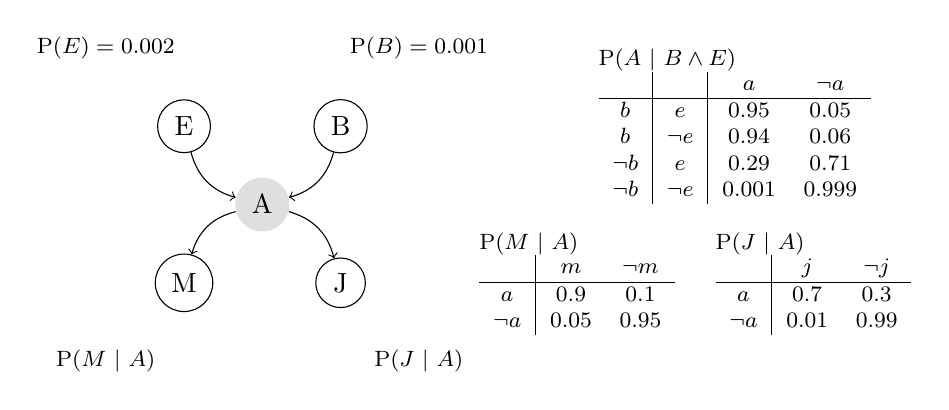
\begin{tikzpicture}[node distance=4em]

            % Nodes
            \node[smodel, circle] (A) {A}; \node[tchoice, above left of=A] (E)
            {E}; \node[above left of=E] {\footnotesize{\(\pr{E}=0.002\)}} ;
            \node[tchoice, above right of=A] (B) {B}; \node[above right of=B]
            {\footnotesize{\(\pr{B}=0.001\)}} ; \node[tchoice, below left of=A]
            (M) {M}; \node[below left of=M] {\footnotesize{\(\pr{M \given A}\)}}
            ; \node[tchoice, below right of=A] (J) {J}; \node[below right of=J]
            {\footnotesize{\(\pr{J \given A}\)}} ;

            % Edges
            \draw[->] (B) to[bend left] (A); \draw[->] (E) to[bend right] (A);
            \draw[->] (A) to[bend right] (M) ; \draw[->] (A) to[bend left] (J);

            %   EDIT: fc Tables
            \node at (4,-1) {\footnotesize
                $
                    \begin{aligned}
                         & \pr{M \given A}                   \\[-0.55em]
                         & \begin{array}{c|cc}
                                        & m    & \neg m \\
                               \hline a & 0.9  & 0.1    \\
                               \neg a   & 0.05 & 0.95\end{array}
                    \end{aligned}
                $};
            \node at (7,-1) {\footnotesize
                $
                    \begin{aligned}
                         & \pr{J \given A}                   \\[-0.55em]
                         & \begin{array}{c|cc}
                                        & j    & \neg j \\
                               \hline a & 0.7  & 0.3    \\
                               \neg a   & 0.01 & 0.99\end{array}
                    \end{aligned}
                $};
            \node at (6,1) {\footnotesize
                $
                    \begin{aligned}
                         & \pr{A \given B \wedge E}                     \\[-0.55em]
                         & \begin{array}{c|c|cc}
                                        &        & a     & \neg a \\
                               \hline b & e      & 0.95  & 0.05   \\
                               b        & \neg e & 0.94  & 0.06   \\
                               \neg b   & e      & 0.29  & 0.71   \\
                               \neg b   & \neg e & 0.001 & 0.999\end{array}
                    \end{aligned}
                $};

        \end{tikzpicture}
    \end{center}
    \caption{The Earthquake, Burglary, Alarm model}
    \label{figure:bea.model}
\end{figure*}

We follow the convention of representing the (upper case) random
variable \(X\) by the (lower case) positive literal \(x\).
%
Considering the probabilities given in \cref{figure:bea.model} we obtain
the following specification:

\begin{equation*}
    \begin{aligned}
        \probfact{b}{0.001} & ,\cr \probfact{e}{0.002} & ,\cr \end{aligned}
    \label{eq:not_so_simple_example}
\end{equation*}

For the table giving the probability \(\pr{M \given A}\) we obtain the
program:

\begin{equation*}
    \begin{aligned}
        \probfact{\condsymb{m}{a}}{0.9} & ,\cr \probfact{\condsymb{m}{\co{a}}}{0.05} & ,\cr m & \clause a \wedge \condsymb{m}{a},\cr m & \clause \neg a \wedge \condsymb{m}{\co{a}}.
    \end{aligned}
\end{equation*}

The latter program can be simplified (abusing notation) by writing
\(\probrule{m}{0.9}{a}\) and \(\probrule{m}{0.05}{\neg a}\).

Similarly, for the probability \(\pr{J \given A}\) we obtain
\begin{equation*}
    \begin{aligned}
        \probrule{j}{0.7}{  & a},      \\
        \probrule{j}{0.01}{ & \neg a},
    \end{aligned}
\end{equation*}

Finally, for the probability \(\pr{A \given B \wedge E}\) we obtain
\begin{equation*}
    \begin{aligned}
        \probrule{a}{0.95}{b \wedge e},                                              &  &  &
        \probrule{a}{0.94}{b \wedge \co{e}},\cr \probrule{a}{0.29}{\co{b} \wedge e}, &  &  &
        \probrule{a}{0.001}{\co{b} \wedge \co{e}}.
    \end{aligned}\label{eq:prA.given.B.and.E}
\end{equation*}

One can then proceed as in the previous subsection and analyze this
example.  The details of such analysis are not given here since they
are analogous, albeit admittedly more cumbersome.

\end{document}

